\documentclass[11pt,a4paper]{article}
\usepackage[utf8]{inputenc}
\usepackage[T1]{fontenc}
\usepackage[french]{babel}
\usepackage[margin=2.3cm]{geometry}
\usepackage{graphicx,booktabs,longtable,array,float,caption,hyperref,xcolor,enumitem,amsmath}
\usepackage{lmodern}
\hypersetup{colorlinks=true,linkcolor=black,urlcolor=blue!50!black}
\setlist{nosep,leftmargin=1.2em}
\captionsetup{font=small}
\graphicspath{{../figures/}}
\newcommand{\FinalModel}{XGBoost}
\newcommand{\NRows}{48\,842}
\newcommand{\NDup}{52}
\newcommand{\PosRate}{23.9}
\newcommand{\PosF}{10.9}
\newcommand{\PosM}{30.4}
\newcommand{\ShareF}{33.1}
\newcommand{\CapZero}{91.7}
\newcommand{\NTrain}{29\,274}
\newcommand{\NVal}{9\,758}
\newcommand{\NTest}{9\,758}
\newcommand{\MissWork}{2799}
\newcommand{\MissOcc}{2809}
\newcommand{\MissCountry}{857}
\newcommand{\TabCV}{Logistic regression & 40 & 0.734 & 0.898 & 0.727 & 0.676 & 0.296 \\
Random forest & 40 & 0.805 & 0.916 & 0.800 & 0.710 & 0.673 \\
XGBoost & 40 & 0.826 & 0.927 & 0.816 & 0.722 & 0.653 \\}
\newcommand{\TabTest}{Baseline (prior) (val.) & 0.239 & 0.500 & 0.000 & -- & 0.000 & 0.500 & 0.182 & -- \\
Logistic regression & 0.740 & 0.902 & 0.681 & 0.597 & 0.794 & 0.813 & 0.105 & 0.654 \\
Random forest & 0.826 & 0.926 & 0.729 & 0.717 & 0.742 & 0.825 & 0.113 & 0.704 \\
\textbf{XGBoost} & 0.845 & 0.936 & 0.741 & 0.706 & 0.779 & 0.839 & 0.105 & 0.722 \\}
\newcommand{\FinPrauc}{0.845}
\newcommand{\FinRocauc}{0.936}
\newcommand{\FinFone}{0.741}
\newcommand{\FinPrecision}{0.706}
\newcommand{\FinRecall}{0.779}
\newcommand{\FinBalancedacc}{0.839}
\newcommand{\FinBrier}{0.105}
\newcommand{\FinEce}{0.106}
\newcommand{\FinThr}{0.653}
\newcommand{\FinFHalf}{0.722}
\newcommand{\FinRecallHalf}{0.877}
\newcommand{\TabParams}{Logistic regression & \footnotesize C=0.373, class\_weight=None \\
Random forest & \footnotesize n\_estimators=250, max\_depth=14, min\_samples\_leaf=5, max\_features=0.5, class\_weight=balanced \\
XGBoost & \footnotesize reweight=True, n\_estimators=450, learning\_rate=0.0472, max\_depth=5, min\_child\_weight=1.42, subsample=0.75, colsample\_bytree=0.488, reg\_lambda=0.351 \\}
\newcommand{\CalBrier}{0.105}
\newcommand{\CalEce}{0.106}
\newcommand{\CalGap}{+0.106}
\newcommand{\CalMeanPred}{0.345}
\newcommand{\CalObs}{0.239}
\newcommand{\CalIsoBrier}{0.084}
\newcommand{\CalIsoEce}{0.011}
\newcommand{\TabCalBins}{1 & 0.002 & 0.000 & +0.002 \\
2 & 0.009 & 0.002 & +0.007 \\
3 & 0.025 & 0.004 & +0.020 \\
4 & 0.057 & 0.021 & +0.036 \\
5 & 0.123 & 0.045 & +0.078 \\
6 & 0.270 & 0.099 & +0.171 \\
7 & 0.485 & 0.245 & +0.240 \\
8 & 0.674 & 0.373 & +0.301 \\
9 & 0.837 & 0.660 & +0.177 \\
10 & 0.972 & 0.945 & +0.027 \\}
\newcommand{\TabFair}{Before & Female & 0.110 & 0.703 & 0.037 & 0.699 & 0.934 \\
Before & Male & 0.341 & 0.793 & 0.143 & 0.708 & 0.838 \\
Before & \textit{overall} & 0.264 & 0.779 & 0.102 & 0.706 & 0.870 \\ \midrule
After & Female & 0.275 & 0.842 & 0.205 & 0.335 & 0.800 \\
After & Male & 0.399 & 0.851 & 0.202 & 0.648 & 0.814 \\
After & \textit{overall} & 0.358 & 0.849 & 0.203 & 0.568 & 0.809 \\ \midrule}
\newcommand{\DpdB}{0.231}
\newcommand{\DprB}{0.323}
\newcommand{\EodB}{0.106}
\newcommand{\FoneB}{0.741}
\newcommand{\AccB}{0.870}
\newcommand{\DpdA}{0.124}
\newcommand{\DprA}{0.689}
\newcommand{\EodA}{0.009}
\newcommand{\FoneA}{0.681}
\newcommand{\AccA}{0.809}
\newcommand{\RaceDpd}{0.180}
\newcommand{\RaceEod}{0.228}
\newcommand{\TabRace}{Amer-Indian-Eskimo & 93 & 0.107 & 0.714 & 0.058 \\
Asian-Pac-Islander & 303 & 0.287 & 0.853 & 0.101 \\
Black & 937 & 0.130 & 0.724 & 0.037 \\
Other & 80 & 0.125 & 0.625 & 0.069 \\
White & 8345 & 0.281 & 0.781 & 0.112 \\}
\newcommand{\TabShap}{1 & \texttt{is\_married} & 0.608 \\
2 & \texttt{log\_capital\_net} & 0.568 \\
3 & \texttt{age\_x\_edu} & 0.561 \\
4 & \texttt{marital-status\_Married-civ-spouse} & 0.434 \\
5 & \texttt{age} & 0.340 \\
6 & \texttt{education-num} & 0.303 \\
7 & \texttt{hours-per-week} & 0.284 \\
8 & \texttt{relationship\_Husband} & 0.157 \\
9 & \texttt{relationship\_Own-child} & 0.138 \\
10 & \texttt{overtime} & 0.127 \\}
\newcommand{\TabShapLocal}{true positive & 1 & 0.657 & \footnotesize \texttt{is\_married} +0.40; \texttt{education-num} -0.32; \texttt{marital-status\_Married-civ-spouse} +0.29; \texttt{hours-per-week} +0.29 \\
true negative & 0 & 0.180 & \footnotesize \texttt{is\_married} -0.65; \texttt{marital-status\_Married-civ-spouse} -0.48; \texttt{age\_x\_edu} +0.40; \texttt{education-num} -0.34 \\
false positive & 0 & 0.776 & \footnotesize \texttt{occupation\_Other-service} -0.70; \texttt{age\_x\_edu} +0.50; \texttt{is\_married} +0.43; \texttt{education-num} +0.41 \\
false negative & 1 & 0.185 & \footnotesize \texttt{age\_x\_edu} -0.86; \texttt{education-num} -0.84; \texttt{is\_married} +0.40; \texttt{occupation\_Machine-op-inspct} -0.37 \\}
\newcommand{\NTrialsTotal}{120}
\newcommand{\TabLog}{0 & 0.7334 & 0.0099 & 0.639 & 3 & 0.7826 & 0.0089 & 0.655 & 6 & 0.8198 & 0.0076 & 0.708 & 8 \\
1 & 0.7335 & 0.0094 & 0.642 & 3 & 0.7980 & 0.0091 & 0.667 & 5 & 0.8212 & 0.0085 & 0.703 & 10 \\
2 & 0.7181 & 0.0100 & 0.603 & 2 & 0.7792 & 0.0078 & 0.667 & 9 & 0.8067 & 0.0072 & 0.670 & 7 \\
3 & 0.7309 & 0.0090 & 0.669 & 3 & 0.7591 & 0.0098 & 0.652 & 8 & 0.8009 & 0.0075 & 0.689 & 3 \\
4 & 0.7333 & 0.0094 & 0.643 & 4 & 0.7875 & 0.0092 & 0.683 & 4 & 0.8061 & 0.0075 & 0.681 & 7 \\
5 & 0.7261 & 0.0098 & 0.667 & 2 & 0.7886 & 0.0104 & 0.687 & 16 & 0.8116 & 0.0075 & 0.689 & 5 \\
6 & 0.7312 & 0.0093 & 0.669 & 3 & 0.7877 & 0.0095 & 0.679 & 8 & 0.7389 & 0.0104 & 0.655 & 3 \\
7 & 0.7233 & 0.0099 & 0.663 & 2 & 0.7715 & 0.0100 & 0.663 & 9 & 0.8191 & 0.0077 & 0.688 & 7 \\
8 & 0.7336 & 0.0097 & 0.642 & 3 & 0.8021 & 0.0087 & 0.693 & 20 & 0.8135 & 0.0078 & 0.709 & 10 \\
9 & 0.7337 & 0.0095 & 0.642 & 4 & 0.7759 & 0.0081 & 0.644 & 4 & 0.7910 & 0.0079 & 0.648 & 4 \\
10 & 0.7332 & 0.0094 & 0.643 & 5 & 0.8018 & 0.0088 & 0.693 & 25 & 0.8044 & 0.0082 & 0.679 & 10 \\
11 & 0.7331 & 0.0100 & 0.639 & 3 & 0.8022 & 0.0088 & 0.692 & 22 & 0.8213 & 0.0078 & 0.710 & 12 \\
12 & 0.7336 & 0.0095 & 0.642 & 4 & 0.7992 & 0.0091 & 0.688 & 19 & 0.8165 & 0.0074 & 0.699 & 11 \\
13 & 0.7336 & 0.0096 & 0.643 & 3 & 0.7990 & 0.0081 & 0.697 & 18 & 0.8221 & 0.0080 & 0.710 & 8 \\
14 & 0.7309 & 0.0102 & 0.631 & 3 & 0.7929 & 0.0084 & 0.662 & 11 & 0.8226 & 0.0076 & 0.709 & 8 \\
15 & 0.7309 & 0.0090 & 0.669 & 4 & 0.7998 & 0.0096 & 0.693 & 21 & 0.8184 & 0.0076 & 0.709 & 10 \\
16 & 0.7334 & 0.0094 & 0.643 & 4 & 0.8033 & 0.0083 & 0.692 & 19 & 0.8165 & 0.0080 & 0.703 & 12 \\
17 & 0.7312 & 0.0090 & 0.669 & 4 & 0.8050 & 0.0082 & 0.698 & 20 & 0.8221 & 0.0070 & 0.710 & 9 \\
18 & 0.7314 & 0.0101 & 0.631 & 3 & 0.8048 & 0.0080 & 0.697 & 27 & 0.8190 & 0.0082 & 0.710 & 10 \\
19 & 0.7334 & 0.0094 & 0.642 & 4 & 0.8021 & 0.0081 & 0.689 & 6 & 0.8236 & 0.0076 & 0.710 & 9 \\
20 & 0.7336 & 0.0097 & 0.641 & 3 & 0.8045 & 0.0083 & 0.696 & 16 & 0.8168 & 0.0078 & 0.703 & 10 \\
21 & 0.7336 & 0.0095 & 0.642 & 4 & 0.8036 & 0.0077 & 0.698 & 15 & 0.8240 & 0.0079 & 0.711 & 11 \\
22 & 0.7300 & 0.0097 & 0.669 & 3 & 0.8048 & 0.0081 & 0.696 & 22 & 0.8194 & 0.0076 & 0.707 & 9 \\
23 & 0.7335 & 0.0094 & 0.642 & 4 & 0.8036 & 0.0082 & 0.699 & 23 & 0.8189 & 0.0083 & 0.709 & 11 \\
24 & 0.7337 & 0.0097 & 0.642 & 3 & 0.8003 & 0.0093 & 0.691 & 12 & 0.8228 & 0.0076 & 0.711 & 10 \\
25 & 0.7336 & 0.0097 & 0.641 & 3 & 0.8027 & 0.0082 & 0.701 & 22 & 0.8211 & 0.0076 & 0.709 & 10 \\
26 & 0.7333 & 0.0093 & 0.643 & 4 & 0.8024 & 0.0083 & 0.678 & 24 & 0.8234 & 0.0079 & 0.712 & 26 \\
27 & 0.7252 & 0.0103 & 0.620 & 2 & 0.7910 & 0.0089 & 0.687 & 11 & 0.8235 & 0.0081 & 0.710 & 38 \\
28 & 0.7335 & 0.0098 & 0.640 & 3 & 0.8000 & 0.0092 & 0.690 & 13 & 0.8227 & 0.0080 & 0.710 & 33 \\
29 & 0.7328 & 0.0100 & 0.637 & 3 & 0.7994 & 0.0087 & 0.695 & 11 & 0.8252 & 0.0076 & 0.713 & 30 \\
30 & 0.7313 & 0.0091 & 0.669 & 4 & 0.7988 & 0.0097 & 0.688 & 14 & 0.8235 & 0.0078 & 0.710 & 36 \\
31 & 0.7336 & 0.0097 & 0.641 & 4 & 0.8001 & 0.0082 & 0.686 & 11 & 0.8229 & 0.0077 & 0.710 & 62 \\
32 & 0.7336 & 0.0098 & 0.640 & 3 & 0.8012 & 0.0083 & 0.691 & 8 & 0.8193 & 0.0076 & 0.706 & 39 \\
33 & 0.7337 & 0.0096 & 0.642 & 4 & 0.7932 & 0.0077 & 0.696 & 20 & 0.8248 & 0.0073 & 0.712 & 35 \\
34 & 0.7336 & 0.0095 & 0.643 & 4 & 0.8049 & 0.0081 & 0.696 & 16 & 0.8230 & 0.0074 & 0.710 & 28 \\
35 & 0.7335 & 0.0095 & 0.643 & 4 & 0.8022 & 0.0082 & 0.692 & 16 & 0.8259 & 0.0073 & 0.713 & 35 \\
36 & 0.7311 & 0.0090 & 0.668 & 4 & 0.8041 & 0.0080 & 0.702 & 25 & 0.8209 & 0.0080 & 0.707 & 38 \\
37 & 0.7332 & 0.0099 & 0.639 & 3 & 0.7748 & 0.0074 & 0.663 & 13 & 0.8253 & 0.0073 & 0.713 & 38 \\
38 & 0.7308 & 0.0091 & 0.668 & 4 & 0.7817 & 0.0096 & 0.676 & 10 & 0.8237 & 0.0074 & 0.712 & 33 \\
39 & 0.7307 & 0.0095 & 0.669 & 3 & 0.7904 & 0.0084 & 0.679 & 21 & 0.8243 & 0.0076 & 0.712 & 36 \\}
\newcommand{\SelFB}{0.110}
\newcommand{\TprFB}{0.703}
\newcommand{\FprFB}{0.037}
\newcommand{\PrecFB}{0.699}
\newcommand{\AccFB}{0.934}
\newcommand{\SelMB}{0.341}
\newcommand{\TprMB}{0.793}
\newcommand{\FprMB}{0.143}
\newcommand{\PrecMB}{0.708}
\newcommand{\AccMB}{0.838}
\newcommand{\SelFA}{0.275}
\newcommand{\TprFA}{0.842}
\newcommand{\FprFA}{0.205}
\newcommand{\PrecFA}{0.335}
\newcommand{\AccFA}{0.800}
\newcommand{\SelMA}{0.399}
\newcommand{\TprMA}{0.851}
\newcommand{\FprMA}{0.202}
\newcommand{\PrecMA}{0.648}
\newcommand{\AccMA}{0.814}
\newcommand{\TestPrLog}{0.740}
\newcommand{\TestRocLog}{0.902}
\newcommand{\TestFoneLog}{0.681}
\newcommand{\CvPrLog}{0.734}
\newcommand{\ValPrLog}{0.727}
\newcommand{\ThrLog}{0.296}
\newcommand{\TestPrRf}{0.826}
\newcommand{\TestRocRf}{0.926}
\newcommand{\TestFoneRf}{0.729}
\newcommand{\CvPrRf}{0.805}
\newcommand{\ValPrRf}{0.800}
\newcommand{\ThrRf}{0.673}
\newcommand{\TestPrXgb}{0.845}
\newcommand{\TestRocXgb}{0.936}
\newcommand{\TestFoneXgb}{0.741}
\newcommand{\CvPrXgb}{0.826}
\newcommand{\ValPrXgb}{0.816}
\newcommand{\ThrXgb}{0.653}
\newcommand{\BasePr}{0.239}
\newcommand{\BaseBrier}{0.182}
\newcommand{\BaseAcc}{0.761}
\newcommand{\FinAcc}{0.870}
\newcommand{\CvStdXgb}{0.014}
\newcommand{\EceLog}{0.009}
\newcommand{\BrierLog}{0.105}
\newcommand{\RealGap}{0.195}
\newcommand{\NCols}{76}
\newcommand{\XOccMissRate}{9.7}
\newcommand{\XOccExecRate}{47.1}
\newcommand{\XOccProfRate}{44.8}
\newcommand{\XOccServRate}{4.2}
\newcommand{\XOccHouseRate}{1.3}
\newcommand{\XRelHusbandRate}{45.0}
\newcommand{\XRelWifeRate}{46.8}
\newcommand{\XRelChildRate}{1.2}
\newcommand{\XTrainPosRate}{23.9}
\newcommand{\XCapGainPosRate}{62.1}
\newcommand{\XCapGainZeroPosRate}{20.6}
\newcommand{\XCapGainShare}{8.1}
\newcommand{\XMissBothShare}{99.8}
\newcommand{\XHusbandMaleShare}{100.0}
\newcommand{\XMarriedMaleShare}{88.8}
\newcommand{\XMaleMarriedRate}{60.7}
\newcommand{\XFemaleMarriedRate}{15.5}
\newcommand{\XTnLog}{6169}
\newcommand{\XFpLog}{1253}
\newcommand{\XFnLog}{481}
\newcommand{\XTpLog}{1855}
\newcommand{\XTnRf}{6736}
\newcommand{\XFpRf}{686}
\newcommand{\XFnRf}{602}
\newcommand{\XTpRf}{1734}
\newcommand{\XTnXgb}{6665}
\newcommand{\XFpXgb}{757}
\newcommand{\XFnXgb}{515}
\newcommand{\XTpXgb}{1821}
\newcommand{\XSweepBestFone}{0.722}
\newcommand{\XSweepFlatLo}{0.56}
\newcommand{\XSweepFlatHi}{0.72}
\newcommand{\XTrialMinLog}{0.718}
\newcommand{\XTrialMedLog}{0.733}
\newcommand{\XTrialMaxLog}{0.734}
\newcommand{\XWithinLog}{36}
\newcommand{\XFoldStdLog}{0.010}
\newcommand{\XTrialMinRf}{0.759}
\newcommand{\XTrialMedRf}{0.800}
\newcommand{\XTrialMaxRf}{0.805}
\newcommand{\XWithinRf}{19}
\newcommand{\XFoldStdRf}{0.008}
\newcommand{\XTrialMinXgb}{0.739}
\newcommand{\XTrialMedXgb}{0.821}
\newcommand{\XTrialMaxXgb}{0.826}
\newcommand{\XWithinXgb}{21}
\newcommand{\XFoldStdXgb}{0.007}
\newcommand{\XLogBestNone}{0.734}
\newcommand{\XLogBestBal}{0.731}
\newcommand{\XXgbBestW}{0.826}
\newcommand{\XXgbBestNoW}{0.821}
\newcommand{\XRfBestNone}{0.802}
\newcommand{\XRfBestBal}{0.805}
\newcommand{\XTimeLog}{3}
\newcommand{\XTimeRf}{15}
\newcommand{\XTimeXgb}{10}
\newcommand{\XAgeCross}{35}
\newcommand{\XEduCross}{12}
\newcommand{\XHoursCross}{45}
\newcommand{\XMarriedShapOn}{+0.42}
\newcommand{\XMarriedShapOff}{-0.75}
\newcommand{\XAucF}{0.959}
\newcommand{\XApF}{0.808}
\newcommand{\XEceF}{0.077}
\newcommand{\XMeanPF}{0.187}
\newcommand{\XObsF}{0.109}
\newcommand{\XMeanPPosF}{0.749}
\newcommand{\XMeanPNegF}{0.117}
\newcommand{\XAucM}{0.918}
\newcommand{\XApM}{0.852}
\newcommand{\XEceM}{0.120}
\newcommand{\XMeanPM}{0.424}
\newcommand{\XObsM}{0.304}
\newcommand{\XMeanPPosM}{0.796}
\newcommand{\XMeanPNegM}{0.261}

\newcommand{\GroupNb}{3}% à confirmer : le planning oral liste ce groupe en n°10

\title{\textbf{Prédire un revenu supérieur à 50\,k\$ : pipeline, réglage, explicabilité, calibration et équité}\\[2pt]
\large Applied ML: Foundations, Engineering \& Evaluation (MSA-DATI07-05)}
\author{Groupe \GroupNb{} : Max GUIRIEC, Amaniel ASRAT, Zackary AICH}
\date{Novembre 2026}

\begin{document}
\maketitle
\vspace{-1.2em}
\begin{center}
\fbox{\parbox{0.92\linewidth}{\centering
\textbf{Dataset utilisé : Option 1 --- Adult / Census Income} (recensement américain de 1994, \NRows{} lignes, 14 variables).\\
\textbf{Dépôt GitHub (code, README, requirements, configuration, journal des essais) :}\\
\url{https://github.com/Maqs-1/applied-ml-adult-income}}}
\end{center}

\section{Cadrage du problème et analyse exploratoire}
\paragraph{Tâche.} Prédire si une personne gagne plus de 50\,k\$ par an (classe positive) à partir de caractéristiques démographiques et professionnelles. Le jeu est chargé via \texttt{fetch\_openml}, avec un repli automatique sur la source UCI d'origine (mêmes \NRows{} lignes) : OpenML renvoyait une erreur 503 au moment du travail.

\paragraph{Ce que montre l'EDA} (Fig.~\ref{fig:eda}). La classe positive représente \PosRate\,\% des lignes : le problème est déséquilibré, et un modèle qui prédit toujours ``$\leq$50K'' obtient déjà \BaseAcc{} d'accuracy (Sec.~\ref{sec:imb}). Les valeurs manquantes sont codées ``?'' et concentrées sur trois colonnes : \texttt{workclass} (\MissWork), \texttt{occupation} (\MissOcc) et \texttt{native-country} (\MissCountry) ; les effectifs manquants de \texttt{workclass} et \texttt{occupation} sont quasi identiques, ce qui suggère qu'elles manquent ensemble ; le manque peut donc être informatif. \CapZero\,\% des personnes ont un gain en capital nul, avec une queue très lourde. Enfin le taux de revenus élevés diffère fortement selon le sexe : \PosF\,\% chez les femmes (\ShareF\,\% de l'échantillon) contre \PosM\,\% chez les hommes, ce qui motivera l'audit d'équité (Sec.~\ref{sec:fair}).

\begin{figure}[htbp]\centering
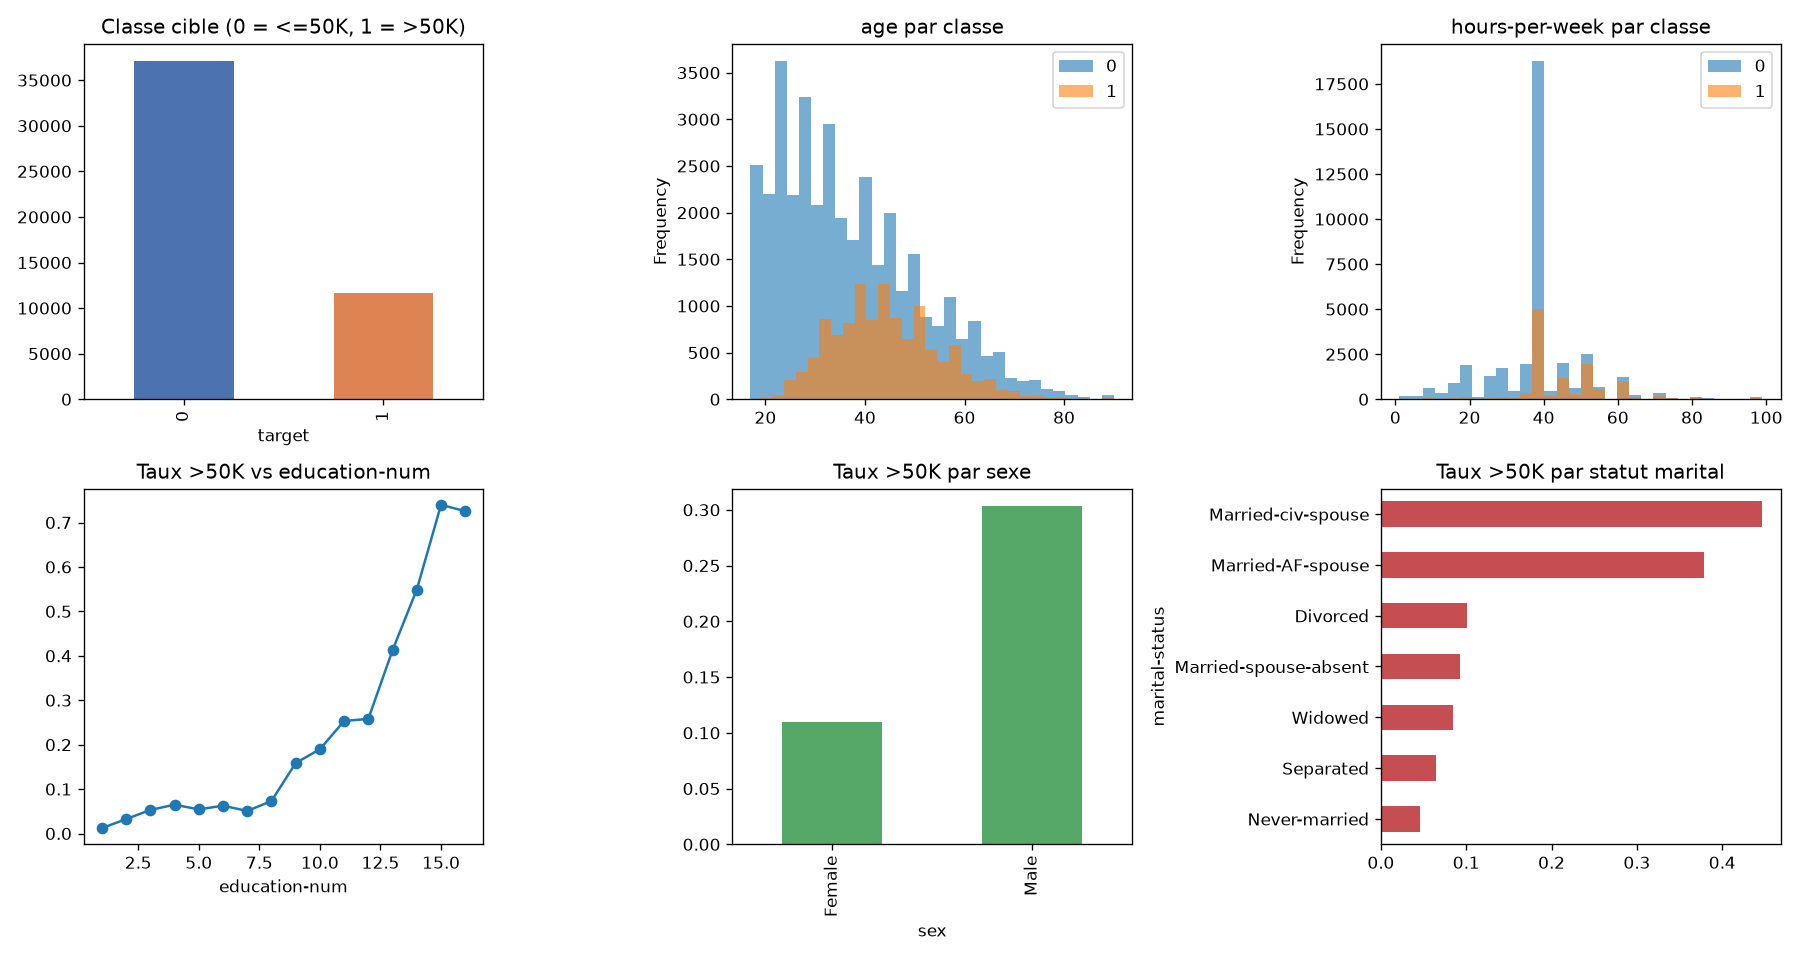
\includegraphics[width=0.85\linewidth]{eda_overview.png}
\caption{Vue d'ensemble : déséquilibre de la cible, distributions d'âge et d'heures, taux de positifs selon le niveau d'études, le sexe et le statut marital.}\label{fig:eda}
\end{figure}

\paragraph{Découpage honnête.} Les \NDup{} doublons exacts sont supprimés \emph{avant} le découpage (sinon une même ligne pourrait être en entraînement et en test). Le découpage 60/20/20, \emph{stratifié sur (cible $\times$ sexe)} avec la graine 42, donne \NTrain{} lignes d'entraînement, \NVal{} de validation et \NTest{} de test, avec la même prévalence dans chacun. Les rôles sont stricts : \textbf{entraînement} = apprentissage et validation croisée d'Optuna ; \textbf{validation} = choix du seuil de décision, du modèle final, de la recalibration et de la mitigation ; \textbf{test} = lu uniquement pour rapporter les résultats finaux, jamais pour décider.

\section{Feature engineering et Pipeline unique}\label{sec:fe}
Tout le prétraitement et le modèle sont dans un seul \texttt{sklearn.pipeline.Pipeline} (\texttt{FeatureEngineer} $\rightarrow$ \texttt{ColumnTransformer} $\rightarrow$ modèle). Il est donc ré-appris dans chaque pli de validation croisée, sans fuite possible.

\paragraph{Valeurs manquantes et encodage.} Variables numériques : imputation par la médiane (et standardisation pour le modèle linéaire seulement). Variables catégorielles : les manquants deviennent une modalité explicite ``Missing'' (le manque est informatif), puis one-hot, avec regroupement des modalités vues moins de 20 fois et gestion des modalités inconnues. On obtient \NCols{} colonnes.

\paragraph{Variables construites (justifiées).}
\begin{itemize}
\item \texttt{log\_capital\_net} : logarithme signé de (gain $-$ perte en capital), pour écraser une distribution à queue très lourde.
\item \texttt{has\_capital} : présence d'un revenu du capital, proxy de patrimoine.
\item \texttt{is\_married} : marié(e) vivant avec son conjoint (7 modalités regroupées en un signal fort : foyer avec deux revenus potentiels).
\item \texttt{overtime} : plus de 40 heures par semaine.
\item \texttt{age\_x\_edu} : interaction âge $\times$ années d'études (expérience valorisée par le diplôme), surtout utile au modèle linéaire.
\end{itemize}
\paragraph{Colonnes retirées.} \texttt{fnlwgt} (poids d'échantillonnage du recensement, pas une caractéristique de la personne) et \texttt{education} (redondante avec \texttt{education-num}). Les attributs sensibles \texttt{sex} et \texttt{race} sont \emph{exclus des entrées du modèle} mais conservés à part pour l'audit ; nous verrons en Sec.~\ref{sec:shap} et~\ref{sec:fair} que cela ne suffit pas à supprimer le biais.

\section{Déséquilibre des classes}\label{sec:imb}
\paragraph{Métriques.} L'accuracy est trompeuse ici : le baseline (prédire toujours la classe majoritaire) atteint \BaseAcc{} avec un rappel nul. Nous retenons la \textbf{PR-AUC} (précision moyenne) comme métrique d'optimisation, car elle se concentre sur la classe rare et ne dépend pas d'un seuil ; son niveau de référence est la prévalence (\BasePr). Nous rapportons aussi ROC-AUC, F1, précision, rappel, accuracy équilibrée et Brier.

\paragraph{Remède et justification.} Nous combinons deux leviers, appliqués dans \texttt{src/train.py} : (i) une \emph{repondération des classes}, traitée comme un hyperparamètre qu'Optuna tranche (\texttt{class\_weight} $\in$ \{aucun, balanced\} pour la régression logistique et le Random Forest ; \texttt{scale\_pos\_weight} égal au rapport négatifs/positifs ou 1 pour XGBoost) ; (ii) un \emph{seuil de décision} choisi sur la validation pour maximiser le F1, au lieu du seuil 0.5. Nous n'avons pas utilisé SMOTE : il fabrique des exemples synthétiques dans un espace mélangeant variables binaires et continues, n'est utile qu'en cas de déséquilibre extrême, et le déséquilibre ici (1 positif pour 3 négatifs) est modéré. Le rééchantillonnage devrait de toute façon vivre dans le pipeline pour ne pas fuiter.

\paragraph{Ce que le réglage a décidé.} La régression logistique choisit \emph{aucune} repondération, le Random Forest \texttt{balanced}, XGBoost \texttt{scale\_pos\_weight} actif (Tab.~\ref{tab:params}, annexe). Le seuil choisi sur la validation vaut \ThrLog{} (logistique, sans repondération : un seuil bas compense), \ThrRf{} (Random Forest) et \ThrXgb{} (XGBoost). Pour XGBoost, passer du seuil 0.5 au seuil de validation fait passer le F1 de test de \FinFHalf{} à \FinFone{} (le rappel baisse de \FinRecallHalf{} à \FinRecall, la précision monte). Un effet secondaire important de la repondération apparaît en Sec.~\ref{sec:cal}.

\section{Modèles, réglage Optuna et journal des essais}
\paragraph{Les trois modèles.} Nous suivons une progression : \emph{baseline} (prévalence) $\rightarrow$ \textbf{régression logistique} (linéaire, interprétable) $\rightarrow$ \textbf{Random Forest} (non-linéarités et interactions, peu sensible au choix des hyperparamètres) $\rightarrow$ \textbf{XGBoost} (boosting, plus expressif mais plus sensible à ses hyperparamètres).

\paragraph{Réglage avec validation croisée.} Pour chaque modèle, Optuna (échantillonneur TPE, graine 42) exécute \textbf{40 essais} qui maximisent la PR-AUC moyenne d'une validation croisée stratifiée à 5 plis \emph{sur l'entraînement uniquement}. Le score rapporté en CV est donc une moyenne sur des plis non vus par l'ajustement de chaque essai. Comme le meilleur essai est sélectionné parmi 40, ce score reste légèrement optimiste : c'est pourquoi la comparaison finale utilise la validation puis le test, jamais les scores de CV seuls. Le meilleur jeu de paramètres est ensuite ré-entraîné sur tout l'entraînement.

\paragraph{Journal des essais (exigence 7).} Chaque essai écrit une ligne dans \texttt{runs/trials\_log.csv} : modèle, numéro, paramètres, moyennes et écart-type des métriques en CV, durée, et fichier d'artefact (courbe d'historique Optuna \texttt{figures/optuna\_<modèle>\_history.png} ; modèle sauvegardé \texttt{models/<modèle>.joblib} pour la ligne du meilleur essai). Les \NTrialsTotal{} essais sont reproduits en annexe.

\begin{table}[H]\centering\small
\begin{tabular}{lrrrrrr}\toprule
Modèle & Essais & PR-AUC CV & ROC-AUC CV & PR-AUC val. & F1 val. & Seuil \\ \midrule
\TabCV \\ \bottomrule
\end{tabular}
\caption{Meilleur essai de chaque modèle : validation croisée sur l'entraînement, puis validation (seuil choisi sur la validation).}\label{tab:cv}
\end{table}

\section{Comparaison des modèles sur le test}
Le modèle final est choisi \emph{avant} de regarder le test, par la PR-AUC de validation : c'est \FinalModel. Les trois modèles sont ensuite évalués une seule fois sur le test, avec le même protocole et le seuil fixé en validation (Tab.~\ref{tab:test}, Fig.~\ref{fig:pr}).

\begin{table}[H]\centering\small
\setlength{\tabcolsep}{4pt}
\begin{tabular}{lcccccccc}\toprule
Modèle & PR-AUC & ROC-AUC & F1 & Préc. & Rappel & Acc. éq. & Brier & F1@0.5 \\ \midrule
\TabTest \\ \bottomrule
\end{tabular}
\caption{Résultats sur le test (\NTest{} lignes), seuil choisi en validation. Le baseline est évalué sur la validation. Le modèle final est en gras.}\label{tab:test}
\end{table}

\begin{figure}[htbp]\centering
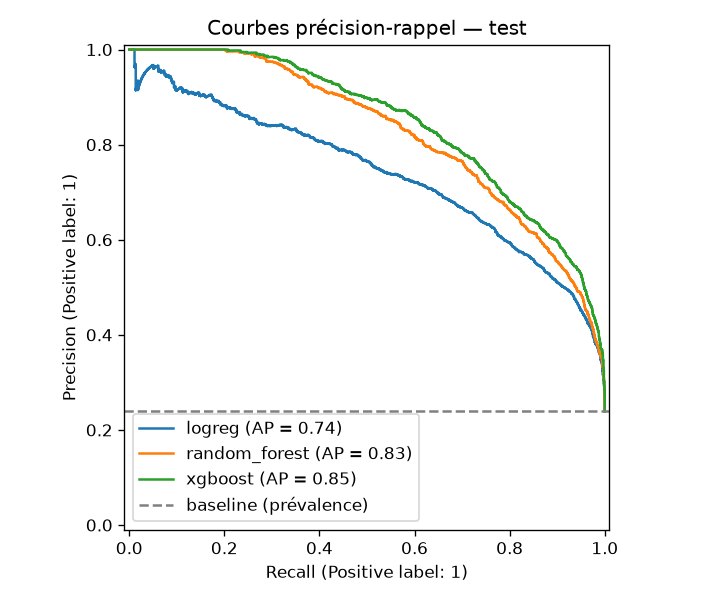
\includegraphics[width=0.58\linewidth]{test_pr_curves.png}
\caption{Courbes précision-rappel sur le test ; la ligne pointillée est la prévalence.}\label{fig:pr}
\end{figure}

\paragraph{Ce que chaque étape apporte.}
\begin{itemize}
\item \emph{Baseline $\rightarrow$ régression logistique} : la PR-AUC passe de \BasePr{} à \TestPrLog{} : les variables (études, âge, statut marital, heures) portent déjà l'essentiel du signal, et le modèle reste entièrement lisible.
\item \emph{Logistique $\rightarrow$ Random Forest} : le gain est le plus fort (PR-AUC \TestPrRf{}, F1 \TestFoneRf{}). Il provient vraisemblablement des interactions et non-linéarités (effet de l'âge, du capital, du statut marital) que la logistique ne capte pas, malgré \texttt{age\_x\_edu} ; nous n'avons pas isolé cette cause par une ablation.
\item \emph{Random Forest $\rightarrow$ XGBoost} : gain plus modeste (PR-AUC \TestPrXgb, ROC-AUC \TestRocXgb), cohérent en CV (\CvPrRf{} $\rightarrow$ \CvPrXgb{}) et en validation (\ValPrRf{} $\rightarrow$ \ValPrXgb). Nous n'avons pas calculé d'intervalles de confiance (limite, Sec.~\ref{sec:lim}) : l'écart RF/XGBoost est petit, et la cohérence sur trois jeux de données est notre seul argument pour le retenir.
\end{itemize}
Le score de test de \FinalModel{} (\TestPrXgb) est supérieur à son score de CV (\CvPrXgb) : cette différence est de l'ordre de la variabilité d'un échantillon de test de cette taille, et ne signale pas de fuite (le test n'a servi à aucun choix) ; nous ne l'interprétons pas davantage.

\section{Explicabilité (SHAP)}\label{sec:shap}
Nous utilisons \texttt{TreeExplainer} sur le pipeline final, appliqué aux variables transformées, sur 1\,000 lignes de test tirées au hasard (graine fixée).

\begin{figure}[htbp]\centering
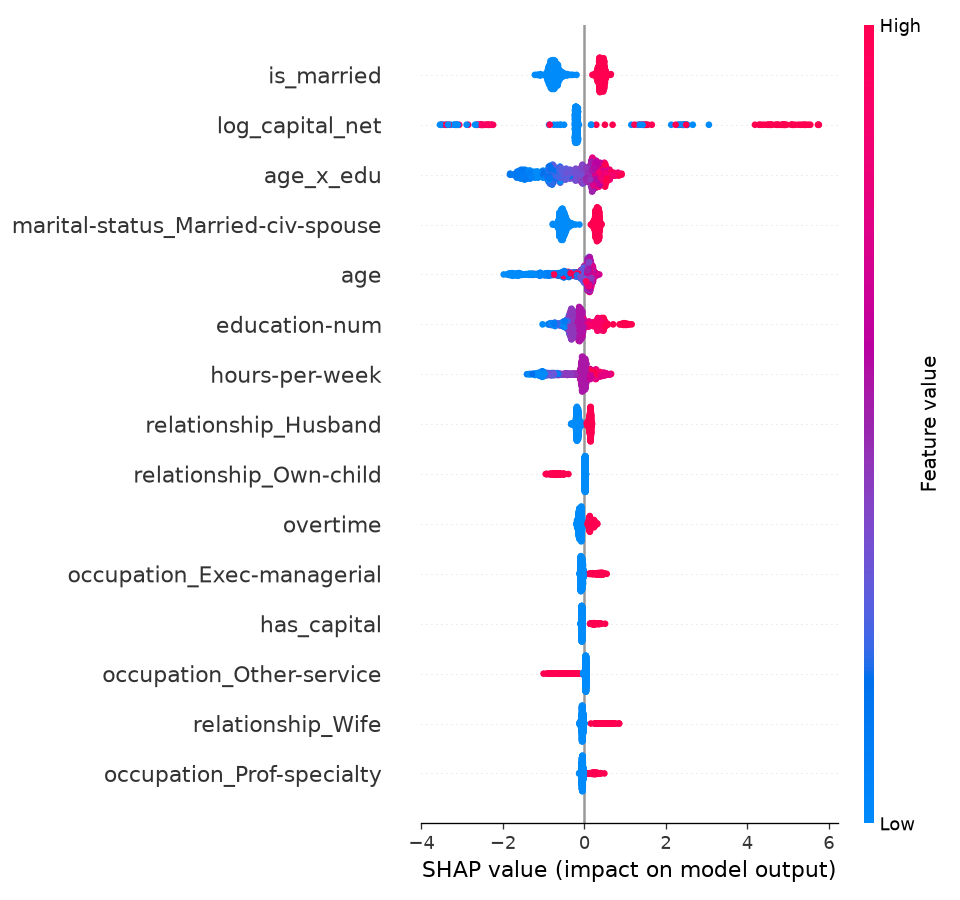
\includegraphics[width=0.78\linewidth]{shap_summary.png}
\caption{Importance globale (SHAP beeswarm) : chaque point est une personne, sa couleur la valeur de la variable.}\label{fig:shap}
\end{figure}

\begin{table}[H]\centering\small
\begin{tabular}{rlr}\toprule
Rang & Variable & Moyenne des $|$SHAP$|$ \\ \midrule
\TabShap \\ \bottomrule
\end{tabular}
\caption{Les dix variables les plus influentes.}\label{tab:shap}
\end{table}

\paragraph{Cohérence métier.} Les variables dominantes sont plausibles : le statut marital (\texttt{is\_married} et \texttt{marital-status\_Married-civ-spouse}, deux encodages quasi identiques dont l'importance se cumule), les gains en capital, le niveau d'études, l'âge/l'expérience et les heures travaillées sont des déterminants classiques du revenu. En revanche, le poids du statut marital est un \emph{signal d'alerte} : dans les données de 1994, un conjoint marié est très souvent un homme chef de foyer (\texttt{relationship\_Husband} figure parmi les dix premières variables). Le modèle peut donc retrouver une partie de l'information sur le sexe à travers des variables corrélées, même sans y avoir accès ; nous n'avons pas mesuré cet effet directement, c'est une hypothèse que l'écart d'équité de la Sec.~\ref{sec:fair} rend crédible.

\paragraph{Explications locales.} Fig.~\ref{fig:local} et Tab.~\ref{tab:local} présentent quatre cas du test : un vrai positif, un vrai négatif, un faux positif et un faux négatif. Sur le faux positif, l'occupation (\texttt{Other-service}) tire la probabilité vers le bas, mais l'effet cumulé du mariage, des études et de l'âge la maintient au-dessus du seuil ; sur le faux négatif, un faible niveau d'études et l'interaction âge $\times$ études dominent alors que la personne gagne plus de 50\,k\$ : le modèle n'a probablement pas accès aux facteurs absents des données (ancienneté, employeur). Les erreurs sont donc cohérentes avec une lecture ``statistique'' du profil.

\begin{figure}[htbp]\centering
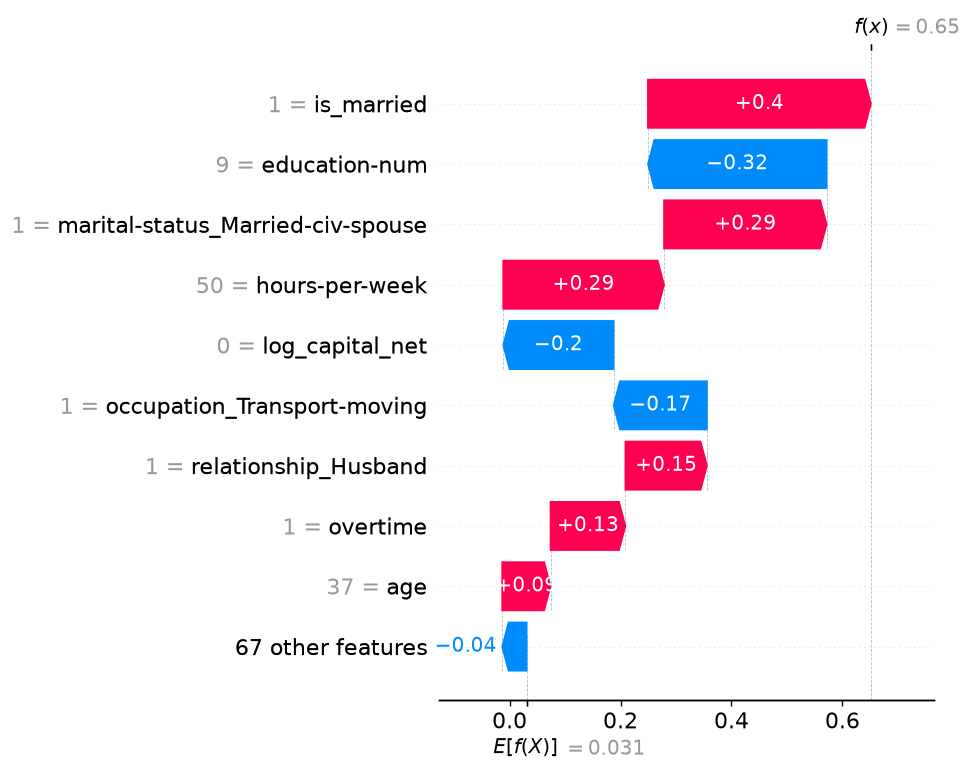
\includegraphics[width=0.48\linewidth]{shap_local_vrai_positif.png}\hfill
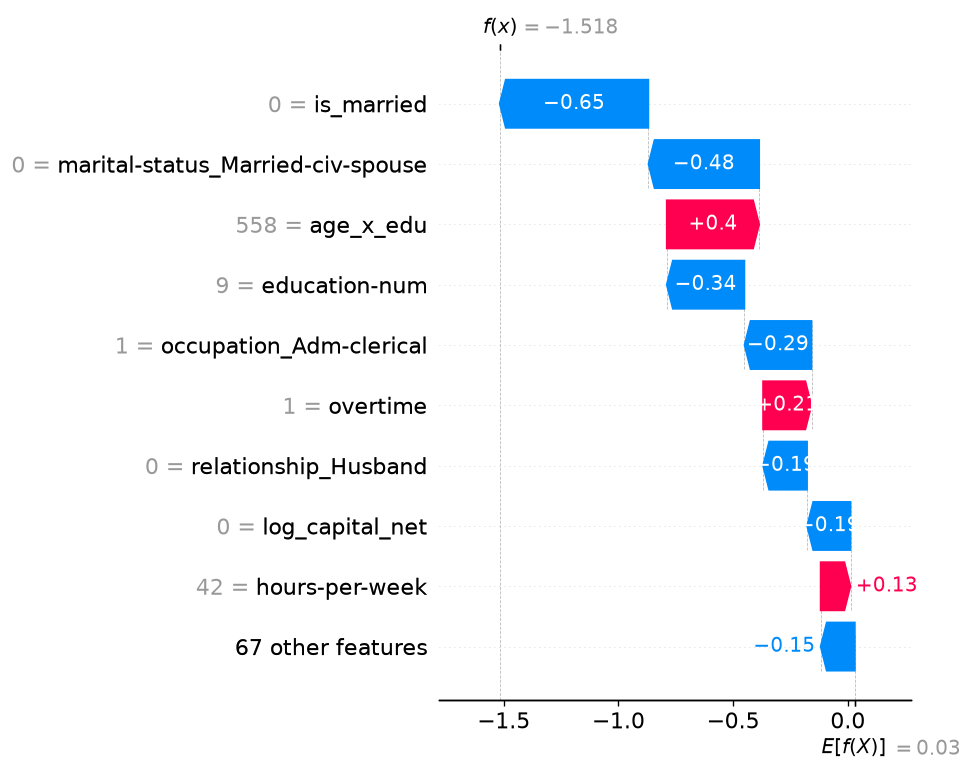
\includegraphics[width=0.48\linewidth]{shap_local_vrai_negatif.png}\\[2pt]
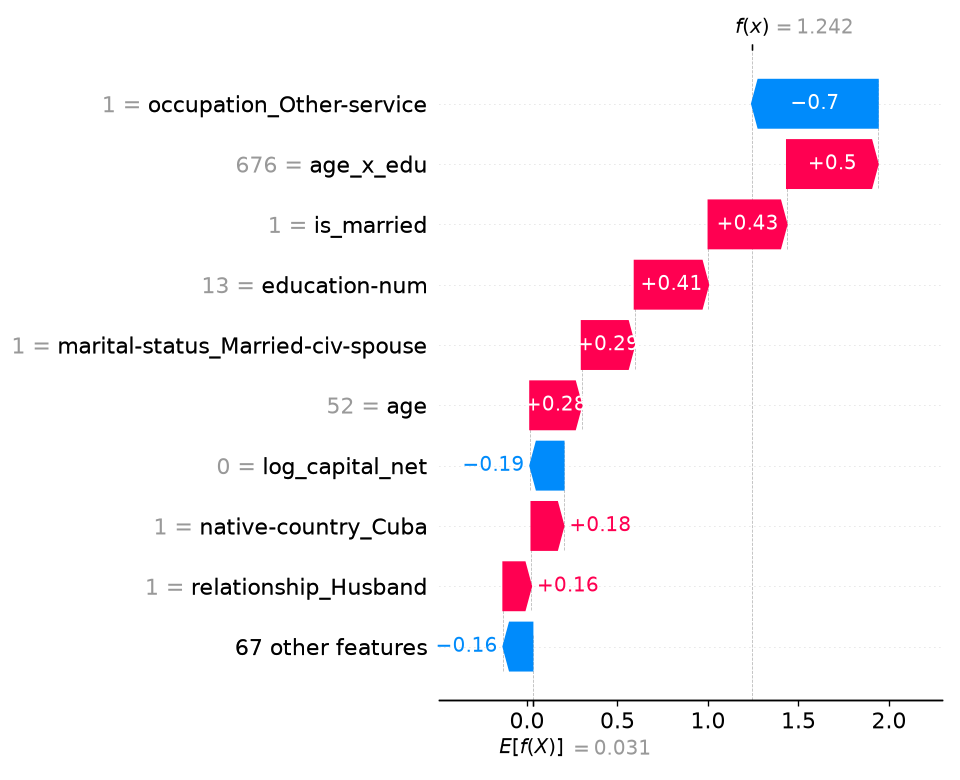
\includegraphics[width=0.48\linewidth]{shap_local_faux_positif.png}\hfill
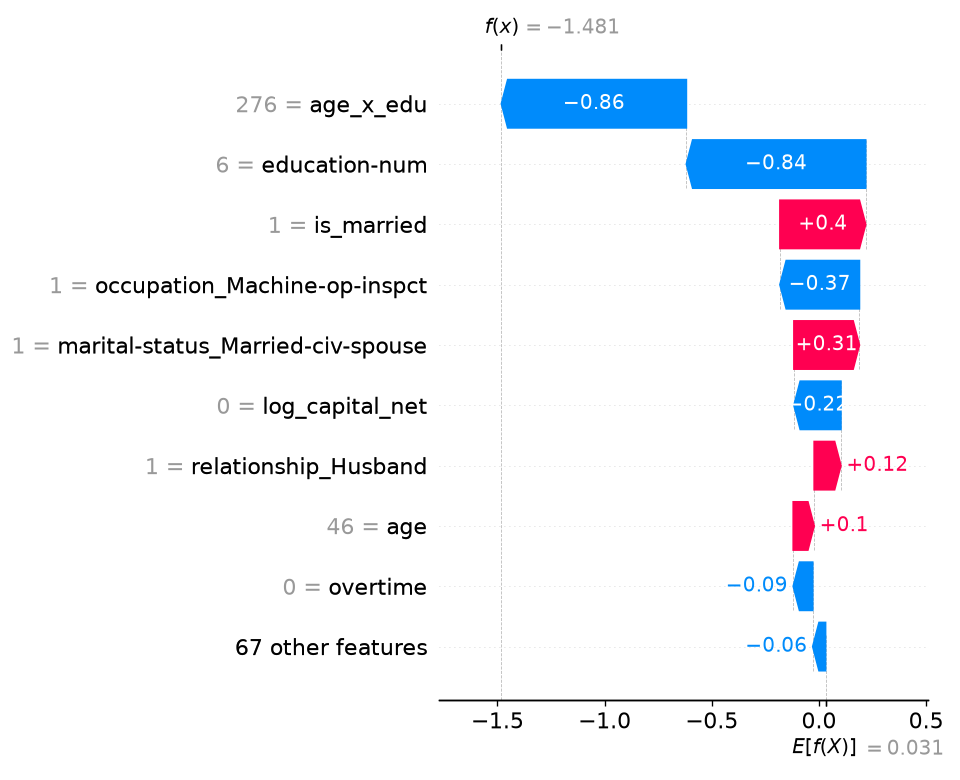
\includegraphics[width=0.48\linewidth]{shap_local_faux_negatif.png}
\caption{Explications locales (waterfall SHAP) : vrai positif, vrai négatif (haut), faux positif, faux négatif (bas).}\label{fig:local}
\end{figure}

\begin{table}[H]\centering\small
\begin{tabular}{lccp{7.4cm}}\toprule
Cas & Vrai & $p(>50\mathrm{K})$ & Principales contributions (SHAP, log-odds) \\ \midrule
\TabShapLocal \\ \bottomrule
\end{tabular}
\caption{Résumé des quatre cas locaux.}\label{tab:local}
\end{table}

\section{Calibration}\label{sec:cal}
\begin{figure}[htbp]\centering
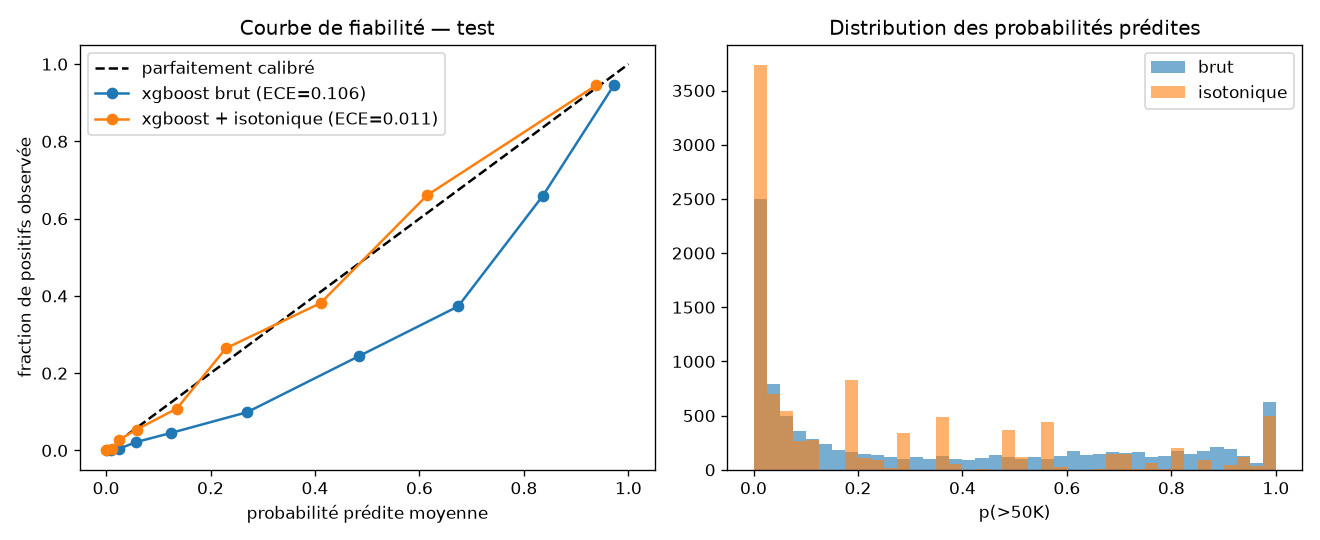
\includegraphics[width=0.93\linewidth]{calibration_reliability.png}
\caption{Courbe de fiabilité de \FinalModel{} sur le test (bacs par quantiles), avant et après recalibration isotonique apprise sur la validation ; distribution des probabilités prédites.}\label{fig:cal}
\end{figure}
\paragraph{Diagnostic.} Le Brier score brut vaut \CalBrier{} et l'ECE \CalEce. La probabilité moyenne prédite est \CalMeanPred{} alors que le taux réel de positifs est \CalObs{} : le modèle \textbf{sur-estime systématiquement la probabilité de la classe positive} (écart moyen \CalGap{}), il est donc ``sur-confiant'' vers les revenus élevés (Fig.~\ref{fig:cal}). La cause est directe : la repondération des classes choisie par Optuna (\texttt{scale\_pos\_weight}) améliore le classement (PR-AUC) mais déplace les probabilités vers le haut. À titre de comparaison, la régression logistique non repondérée est bien mieux calibrée (ECE de \EceLog{} contre \CalEce{} ; leurs Brier sont proches, \BrierLog{} contre \FinBrier), mais son classement est nettement moins bon (Tab.~\ref{tab:test}).
\paragraph{Correctif et décision.} Une recalibration isotonique apprise sur la validation (modèle de base gelé) ramène l'ECE à \CalIsoEce{} et le Brier à \CalIsoBrier{} sur le test. \textbf{Nous ne ferions pas confiance aux probabilités brutes pour une décision aval} (par exemple un seuil de coût, un tarif ou un classement par probabilité absolue) ; en revanche, pour un simple \emph{classement} ou une décision avec le seuil appris, le modèle brut convient, car le seuil a été choisi sur ses sorties brutes. Pour exploiter les probabilités, il faut utiliser la version recalibrée (\texttt{models/<modèle>\_isotonic.joblib}).

\section{Audit d'équité et mitigation}\label{sec:fair}
\paragraph{Attribut sensible et définitions.} L'attribut est le \textbf{sexe} (race en analyse secondaire). Deux définitions sont comparées : la \emph{parité démographique} (le taux de prédictions positives $P(\hat Y=1\mid A)$ est le même entre groupes) et l'\emph{equalized odds} (mêmes TPR et FPR entre groupes, i.e.\ à revenu réel donné, la même chance d'être bien ou mal classé). Les taux de base réels diffèrent (\PosF\,\% contre \PosM\,\%) : exiger la parité démographique reviendrait à ignorer un signal réel et à créer des erreurs différentes selon les groupes, c'est pourquoi la \textbf{mitigation vise l'equalized odds}.

\paragraph{Audit avant mitigation} (test, Tab.~\ref{tab:fair}). Le taux de sélection est de \SelFB{} pour les femmes et \SelMB{} pour les hommes (écart de parité démographique \DpdB, ratio \DprB). Le TPR est de \TprFB{} contre \TprMB{}, et le FPR de \FprFB{} contre \FprMB{} : l'écart d'equalized odds vaut \EodB. Le modèle est donc plus généreux avec les hommes, à la fois en vrais et en faux positifs. Une partie de l'écart de sélection reflète la différence réelle des taux de base, et le modèle la dépasse légèrement (écart de sélection \DpdB{} contre un écart réel de \RealGap{} entre les taux de base). Analyse secondaire sur la race : écart de parité démographique \RaceDpd{} et d'equalized odds \RaceEod{} (Tab.~\ref{tab:race}), à lire avec prudence car certains groupes sont petits.

\paragraph{Mitigation.} Nous appliquons \texttt{ThresholdOptimizer} de Fairlearn (post-traitement, contrainte \texttt{equalized\_odds}) sur le modèle gelé : il apprend, \emph{sur la validation}, un seuil (éventuellement randomisé) par groupe. Il est évalué une seule fois sur le test. Avantages : le modèle n'est pas ré-entraîné et la contrainte est ciblée ; inconvénients : il \emph{utilise le sexe à l'inférence} (ce qui peut poser problème légalement) et ses prédictions sont randomisées (graine fixée).

\begin{table}[H]\centering\small
\begin{tabular}{llccccc}\toprule
Phase & Groupe & Sélection & TPR & FPR & Précision & Accuracy \\ \midrule
\TabFair \bottomrule
\end{tabular}
\caption{Métriques par sexe sur le test, avant et après ThresholdOptimizer.}\label{tab:fair}
\end{table}

\begin{figure}[htbp]\centering
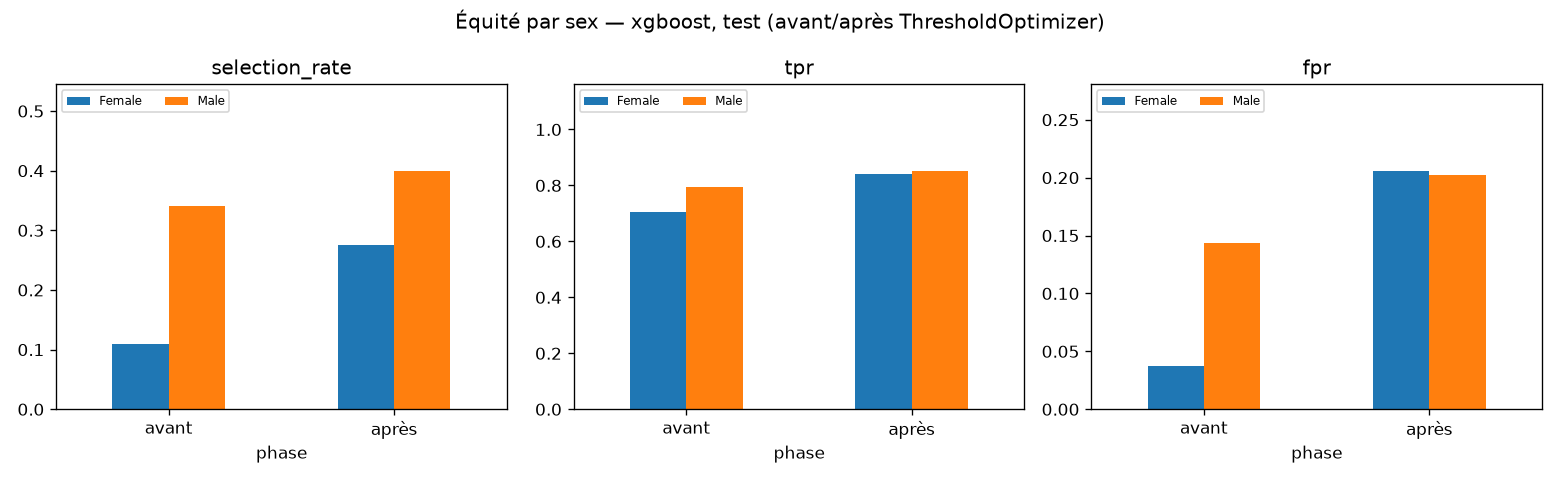
\includegraphics[width=0.93\linewidth]{fairness_before_after.png}
\caption{Taux de sélection, TPR et FPR par sexe, avant et après mitigation (test).}\label{fig:fair}
\end{figure}

\begin{table}[H]\centering\small
\begin{tabular}{lrccc}\toprule
Groupe (race) & Effectif & Sélection & TPR & FPR \\ \midrule
\TabRace \\ \bottomrule
\end{tabular}
\caption{Audit secondaire par race, avant mitigation (test).}\label{tab:race}
\end{table}

\paragraph{Résultat avant/après.} L'écart d'equalized odds tombe de \EodB{} à \EodA{} : l'objectif est atteint. La parité démographique ne l'est pas (\DpdB{} $\rightarrow$ \DpdA), ce qui est attendu puisque les taux de base diffèrent. Mais le coût est réel : le F1 global passe de \FoneB{} à \FoneA{} et l'accuracy de \AccB{} à \AccA. La raison est visible dans le Tab.~\ref{tab:fair} : la contrainte est satisfaite en \emph{rendant le modèle bien plus permissif avec les femmes} (sélection \SelFB{} $\rightarrow$ \SelFA, FPR \FprFB{} $\rightarrow$ \FprFA), si bien que leur précision s'effondre de \PrecFB{} à \PrecFA. Autrement dit, l'égalité des taux d'erreur est obtenue en multipliant les faux positifs chez les femmes. Que ce compromis soit acceptable dépend du coût des faux positifs dans l'usage visé ; sans ce contexte, nous ne recommandons ni l'un ni l'autre des deux modèles, nous documentons le compromis.

\section{Reproductibilité, limites et honnêteté méthodologique}\label{sec:lim}
\paragraph{Reproductibilité.} Graine 42 partout, versions épinglées dans \texttt{requirements.txt} (Python 3.12), paramètres dans \texttt{config.yaml}, une commande pour tout relancer (\texttt{python run\_all.py}). Tous les chiffres de ce rapport sont générés par \texttt{report/gen\_numbers.py} à partir des fichiers \texttt{runs/*.json} produits par le code ; aucun n'est saisi à la main. Un endpoint de prédiction FastAPI (\texttt{src/api.py}) sert le modèle final.
\paragraph{Limites.}
\begin{itemize}
\item Un seul découpage et aucun intervalle de confiance (pas de bootstrap) : les petits écarts, notamment RF contre XGBoost, ne sont pas testés statistiquement.
\item Les résultats du test ont servi à \emph{rapporter} SHAP, calibration et équité, mais aucune décision (hyperparamètres, seuil, modèle, recalibration, mitigation) n'a été prise sur le test.
\item Données de 1994 : la cible et les inégalités qu'elle reflète sont historiques ; l'audit d'équité illustre une méthode, il ne valide pas un usage réel. Nous n'auditons qu'un attribut binaire et une analyse secondaire.
\item Optuna optimise la PR-AUC seule ; la calibration n'est pas dans l'objectif, d'où la sur-confiance observée.
\item Une première exécution complète a dû être refaite : un garde-fou de temps trop court avait interrompu le réglage de XGBoost ; seuls les résultats de la seconde exécution, complète (40 essais par modèle), figurent ici.
\end{itemize}

\section*{Utilisation d'une IA}
Nous avons utilisé \textbf{Claude Code} (Anthropic) comme assistant de développement : écriture et débogage des scripts Python du dépôt, génération du squelette du rapport LaTeX et de la préparation de l'oral. Toutes les valeurs numériques du rapport proviennent de l'exécution du code (génération automatique) et non de l'IA. Les choix méthodologiques exposés ci-dessus sont décrits pour que chaque membre puisse les expliquer et les défendre.

\section*{Déclaration de contribution}
\begin{center}\small
\begin{tabular}{p{3.9cm}p{5.4cm}p{5.6cm}}\toprule
Membre & Responsabilité (défense orale) & Étapes du pipeline \\ \midrule
Max GUIRIEC & Données, EDA, features, pipeline ; coordination Git et rapport & Exigences 1, 2, 5 ; assemblage du dépôt \\
Amaniel ASRAT & Modélisation et réglage & Exigences 3, 4, 6, 7 (déséquilibre, modèles, Optuna, journal) \\
Zackary AICH & Interprétation, calibration, équité & Exigences 8, 9, 10 (SHAP, calibration, audit) \\ \bottomrule
\end{tabular}
\end{center}
Le code a été produit avec l'assistance de Claude Code (voir ci-dessus) ; chaque membre répond de l'ensemble du projet.

\clearpage
\appendix
\section{Hyperparamètres retenus}
\begin{table}[H]\centering
\begin{tabular}{lp{11cm}}\toprule
Modèle & Meilleurs paramètres (essai de meilleure PR-AUC en CV) \\ \midrule
\TabParams \\ \bottomrule
\end{tabular}
\caption{Hyperparamètres des modèles finaux.}\label{tab:params}
\end{table}

\section{Historique des essais Optuna}
\begin{figure}[htbp]\centering
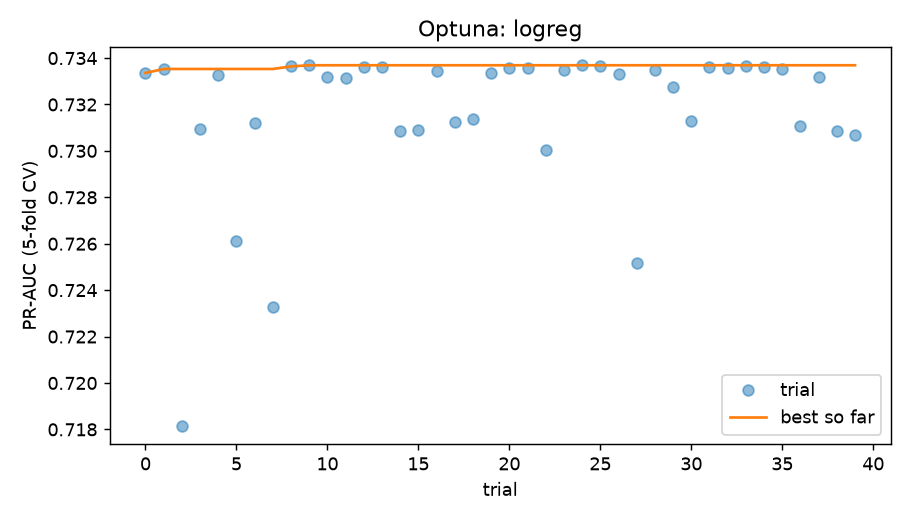
\includegraphics[width=0.32\linewidth]{optuna_logreg_history.png}\hfill
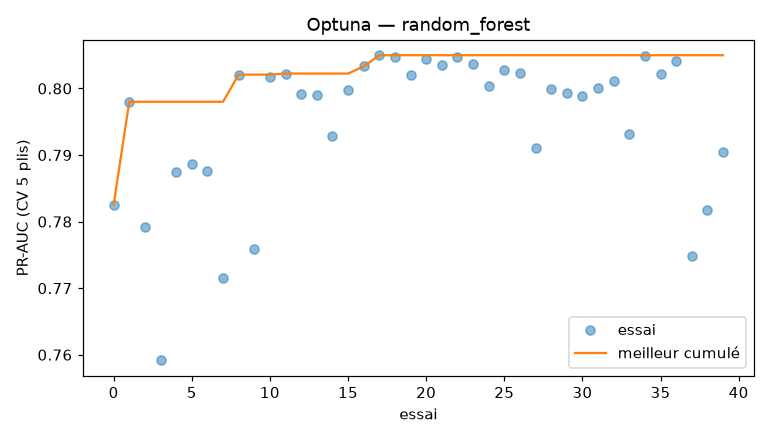
\includegraphics[width=0.32\linewidth]{optuna_random_forest_history.png}\hfill
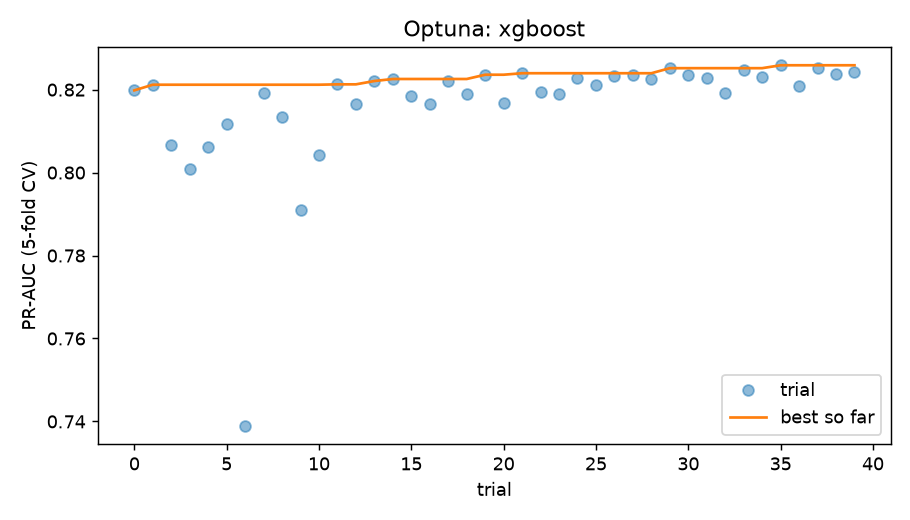
\includegraphics[width=0.32\linewidth]{optuna_xgboost_history.png}
\caption{PR-AUC en CV par essai et meilleur score cumulé, pour chaque modèle.}
\end{figure}

\section{Journal complet des essais (\NTrialsTotal{} essais)}
Colonnes : modèle, numéro d'essai, PR-AUC moyenne et écart-type sur les 5 plis, ROC-AUC, F1, durée (s). Les paramètres de chaque essai et l'artefact associé figurent dans \texttt{runs/trials\_log.csv}.
{\small
\begin{longtable}{lrrrrrr}\toprule
Modèle & Essai & PR-AUC & Écart-type & ROC-AUC & F1 & Durée \\ \midrule\endhead
\TabLog \\ \bottomrule
\end{longtable}}
\end{document}
